\secnumbersection{PROPUESTA DE SOLUCIÓN}

% En esta sección (??)

\subsection{Metodología de trabajo}

Para nuestro proyecto, buscaremos utilizar una metodología de trabajo orientada a la agilidad. Existen multiples metodologias de este estilo, pero hemos decidido utilizar el ciclo \textit{PDCA}\footnote{PDCA: Del inglés Planear, Hacer, Verificar, Actuar.} (\textit{Plan}, \textit{Do}, \textit{Check}, \textit{Act}) por las siguientes razones.

\begin{itemize}
    \item \textbf{Simple}. Nuestro mayor motivo es que consiste en un proceso simple, directo e intuitivo que podemos adoptar e implementar en nuestro flujo de trabajo, desarrollo e implementación de la solución.
    \item \textbf{Cilcico}. Debido a la naturaleza ciclica e iterativa, \textit{PDCA} nos permite identificar las causas de los posibles errores durante el proceso de desarrollo del proyecto. Además, a medida que se implementan distintas soluciones es posible obtener información y experiencia para comprender el proceso que se busca mejorar.
    \item \textbf{Adaptable}. Esta metodología es una estrategia muy adaptable, aquellas personas que decidan implementarla puede decidir con total libertad que aspectos se deben considerar en cada una de las etapas del ciclo, la unica condición es que las definiciones se deben mantener a lo largo de todo el proceso. Esta adaptabilidad permite que \textit{PDCA} sea altamente esacalable, ya que se puede adaptar a cualquier situación y en organizaciones de cualquier tamaño, incluso, en equipos de una sola persona.
\end{itemize}

\begin{figure}[ht]
    \centering
    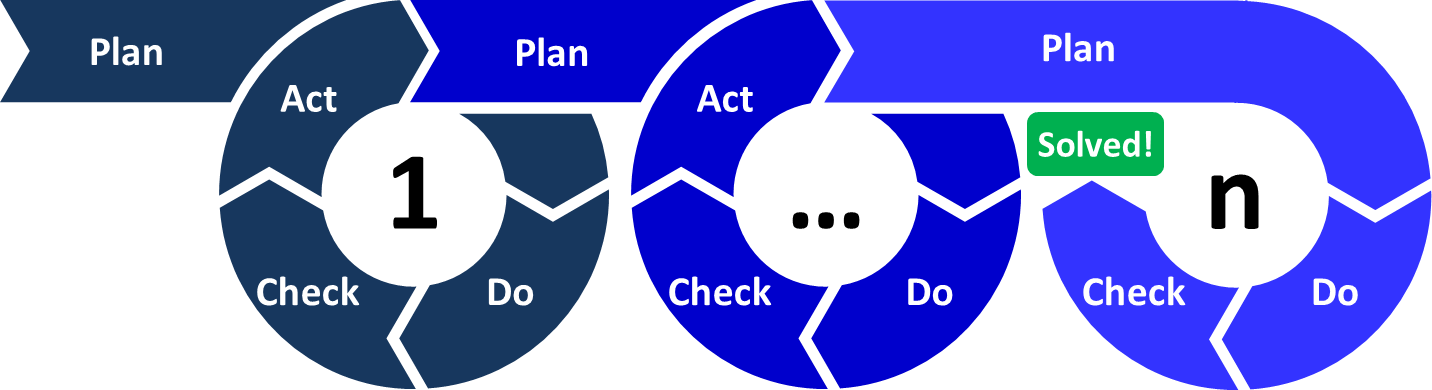
\includegraphics[width=\linewidth]{PDCA-Multi-Loop.png}
    \caption{Ciclos \textit{PDCA}.} Multiples iteraciones del ciclo \textit{PDCA} son realizadas hasta que se logra resolver el problema. Fuente: \textit{PDCA - Wikipedia Commons}.
    \label{fig:pdca-cycle}
\end{figure}

En su esencia \textit{PDCA} es una filosofía para abordar problemas. Primero, identificamos el problema y establecemos nuestros objetivos. Luego, probamos distintos enfoques para alcanzar dichos objetivos, analiszamos nuestros resultados y adaptamos nuestro comportamiento en base a estos. Finalmente, avanzamos la iteración utilizando la solución que ha funcionado.
% TODO: FIXME: REF to https://www.dropbox.com/es/business/resources/pdca

Cada ciclo \textit{PDCA} consiste en las siguientes etapas.

\begin{itemize}
    \item \textbf{Planear}. Debemos comprender nuestro estado actual y el estado deseado. En pocas palabras, esta estapa busca que definamos nuestros objetivos, el cómo alcanzarlos y cómo medir nuestro progreso hacia dichos objetivos.
    \item \textbf{Hacer}. Una vez que hemos definido un plan de acción o una potencial solución para un problema, debemos probarla. Este paso es donde debemos poner a prueba los cambios propuestos en la etapa Planear. Sin embargo, esto se debe considerar como un experimento, no como una solución final. Por lo tanto, todas las pruebas se deben realizar en entornos controlados y a pequeña escala.
    \item \textbf{Verificar}. Luego de completar nuestras pruebas, debems comprobar que los cambios o soluciones propuestas tienen el efecto deseado. En esta etapa se debe analizar la información recopilada durante la etapa Hacer y comparar lo obtenido con los objetivos y metas originales. En resumen, debemos evaluar nuestro nivel de éxito y qué cosas vamos a conservar para el siguiente paso del ciclo.
    \item \textbf{Actuar}. Al llegar a esta etapa, ya hemos logrado identificar una solución o propuesta de cambio para implementar en nuestro problema o proceso. Se deben aplicar estos cambios en la escala que sea necesaria por el proceso y con esto se definen las bases para una nueva iteración.
\end{itemize}

\subsection{Plan de trabajo}

A

\subsection{Analisis inicial}

A

\subsection{Primera iteración: Mejoras al rendimiento general}

A

\subsubsection{Proceso}

A

\subsubsection{Componentes}

A

\subsection{Etapas del sistema}

A

\subsubsection{Etapa de preparación}

A

\subsubsection{Etapa de ranking}

A

\subsubsection{Etapa de indexación}

A

\subsubsection{Etapa de benchmark}

A

\subsubsection{Etapa de servicio}

A

\subsection{Diseño inicial de arquitectura}

A

\subsection{Implementación inicial}

A

\subsection{Resultados}

A

\subsection{Segunda iteración: Desacople de componentes y FlatBuffers}

A

\subsubsection{Diseño}

A

\subsubsection{Implementación}

A

\subsubsection{Resultados}

A

\subsection{Tercera iteración: Paralelización de etapas}

A

\subsubsection{Diseño}

A

\subsubsection{Implementación}

A

\subsubsection{Resultados}

A

\subsection{Cuarta iteración: Actualización de resultados en tiempo real}

A

\subsubsection{Diseño}

A

\subsubsection{Implementación}

A

\subsubsection{Resultados}

A

\subsection{Quinta iteración: Implementación de pruebas}

A

\subsubsection{Planificación}

\subsubsection{Implementación}

\subsubsection{Resultados}

